\section{Results}

\subsection{Protocol-Split Success Rates}

The strong-wind evaluation separates single-goal mission execution from
goal-reissue stress. This protocol split is important because the same method
can behave differently when the system receives one goal command versus
repeated post-arrival or reference-update stimuli. We therefore report
strict-valid counts separately for the single-goal mission protocol
(goal repeat = 1) and the goal-reissue stress protocol
(goal repeat = 10), rather than collapsing the two settings into a
single combined aggregate.

In the single-goal mission protocol, the strongest method in the evaluated set
is the heuristic Wind-Level 0.85, which achieves 26/30 strict-valid runs. The
learned / risk-conditioned methods Risk Adapter v1 and Risk Adapter v2.1 are
both competitive in this setting, each achieving 25/30 strict-valid runs. In
the goal-reissue stress protocol, the ranking changes: Fixed Scale 0.80 is
strongest with 24/30 strict-valid runs, Risk Adapter v1 follows with 23/30, and
Risk Adapter v2.1 drops to 20/30.

\begin{table*}[t]
\centering
\caption{Protocol-split strict-valid counts and balanced robustness metrics.
Counts are strict-valid runs over 30 repeats per protocol. Total regret is
relative to the observed protocol oracles: Wind-Level 0.85 for the single-goal
mission protocol and Fixed Scale 0.80 for the goal-reissue stress protocol.
Counts are descriptive and are not a statistical-significance claim.}
\label{tab:protocol_balanced_robustness}
\resizebox{\linewidth}{!}{%
\begin{tabular}{lcccccl}
\toprule
Method & Single-goal & Stress & Mean & Worst & Total regret & Role \\
\midrule
Original & 21/30 & 18/30 & 19.5/30 & 18/30 & 11 & unadapted baseline \\
Fixed Scale 0.85 & 22/30 & 18/30 & 20.0/30 & 18/30 & 10 & fixed static baseline \\
Wind-Level 0.85 & 26/30 & 16/30 & 21.0/30 & 16/30 & 8 & single-goal specialist heuristic \\
Fixed Scale 0.80 & 21/30 & 24/30 & 22.5/30 & 21/30 & 5 & goal-reissue stress specialist \\
Risk Adapter v1 & 25/30 & 23/30 & 24.0/30 & 23/30 & 2 & balanced learned governor \\
Risk Adapter v2.1 & 25/30 & 20/30 & 22.5/30 & 20/30 & 5 & strong nominal variant \\
\bottomrule
\end{tabular}%
}
\end{table*}


\subsection{Balanced Robustness and Protocol Regret}

Balanced robustness is evaluated using the complete cross-protocol matrix. The
protocol oracles are the highest observed method in each protocol:
Wind-Level 0.85 with 26/30 in the single-goal mission protocol and Fixed Scale
0.80 with 24/30 in the goal-reissue stress protocol. Protocol
regret measures how far each method falls below these observed oracles.

Under this view, Risk Adapter v1 has the strongest balanced performance. It
achieves a mean valid count of 24.0/30, the highest worst-protocol count of
23/30, and the lowest total regret of 2. This is the main reason for centering
Risk Adapter v1 as the paper's balanced learned / risk-conditioned execution
governor.

\begin{figure}[t]
  \centering
  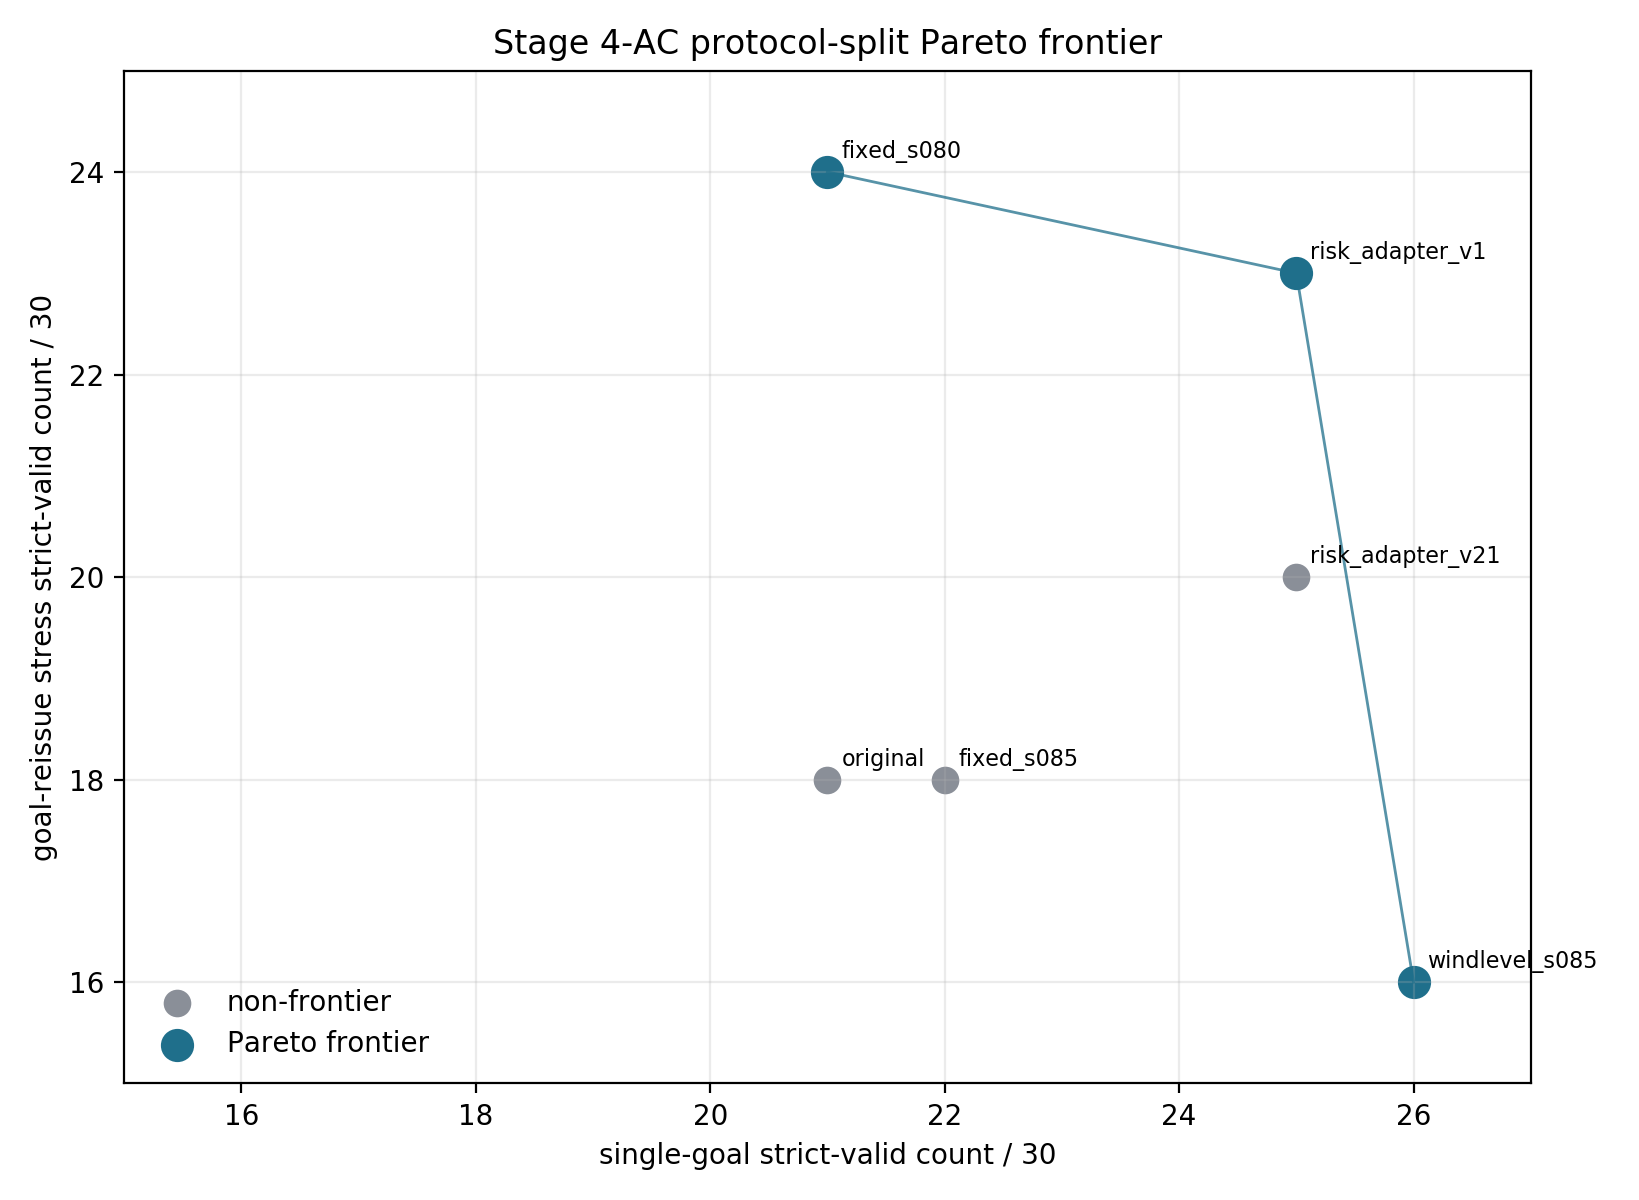
\includegraphics[width=\linewidth]{figures/fig3_pareto.png}
  \caption{Balanced robustness / Pareto frontier across the two tested
  protocols. The x-axis is single-goal strict-valid count / 30 and the y-axis
  is goal-reissue stress strict-valid count / 30. The observed frontier contains
  Wind-Level 0.85, Fixed Scale 0.80, and Risk Adapter v1; this frontier is
  limited to the evaluated methods and protocols.}
  \label{fig:pareto}
\end{figure}

\begin{figure}[t]
  \centering
  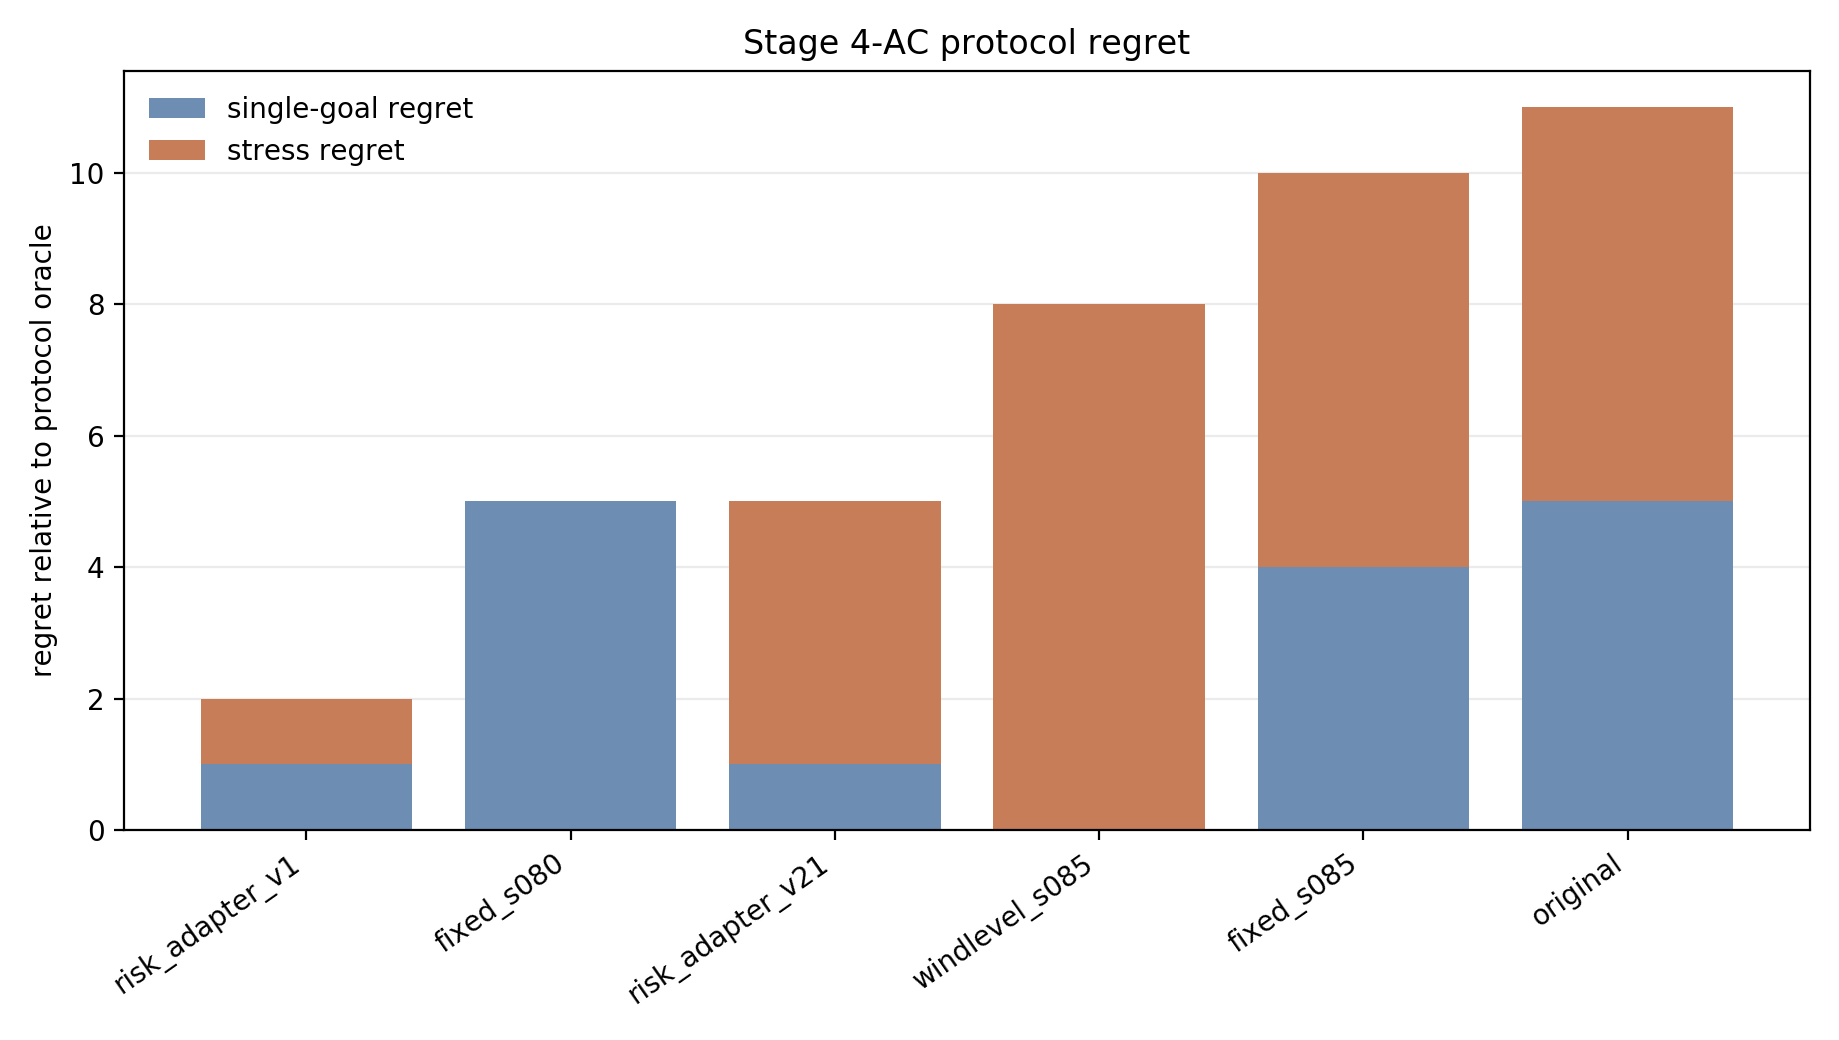
\includegraphics[width=\linewidth]{figures/fig4_protocol_regret.png}
  \caption{Protocol regret relative to the observed protocol oracles.
  Risk Adapter v1 has the lowest total regret under the tested protocols. The
  oracle in each protocol is the observed protocol leader, not a theoretical
  optimum.}
  \label{fig:regret}
\end{figure}

The specialist baselines expose the trade-off that a single protocol would
hide. Wind-Level 0.85 reaches the single-goal oracle with 26/30 but falls to
16/30 under stress. Conversely, Fixed Scale 0.80 reaches the stress oracle with
24/30 but achieves only 21/30 in the single-goal mission protocol. Risk Adapter
v2.1 is not on the observed Pareto frontier because it has the same single-goal
count as Risk Adapter v1 (25/30) but a lower stress count (20/30 versus 23/30).

\subsection{Failure-Mode-Aware Diagnosis}

Protocol-split success counts explain which methods are stronger, but they do
not explain how invalid runs occur. We therefore use invalid-only failure
groups as a diagnostic view. These labels should be read as failure-analysis
categories, not definitive root-cause attribution; the paper-facing success
metric remains strict-valid count.

\begin{figure}[t]
  \centering
  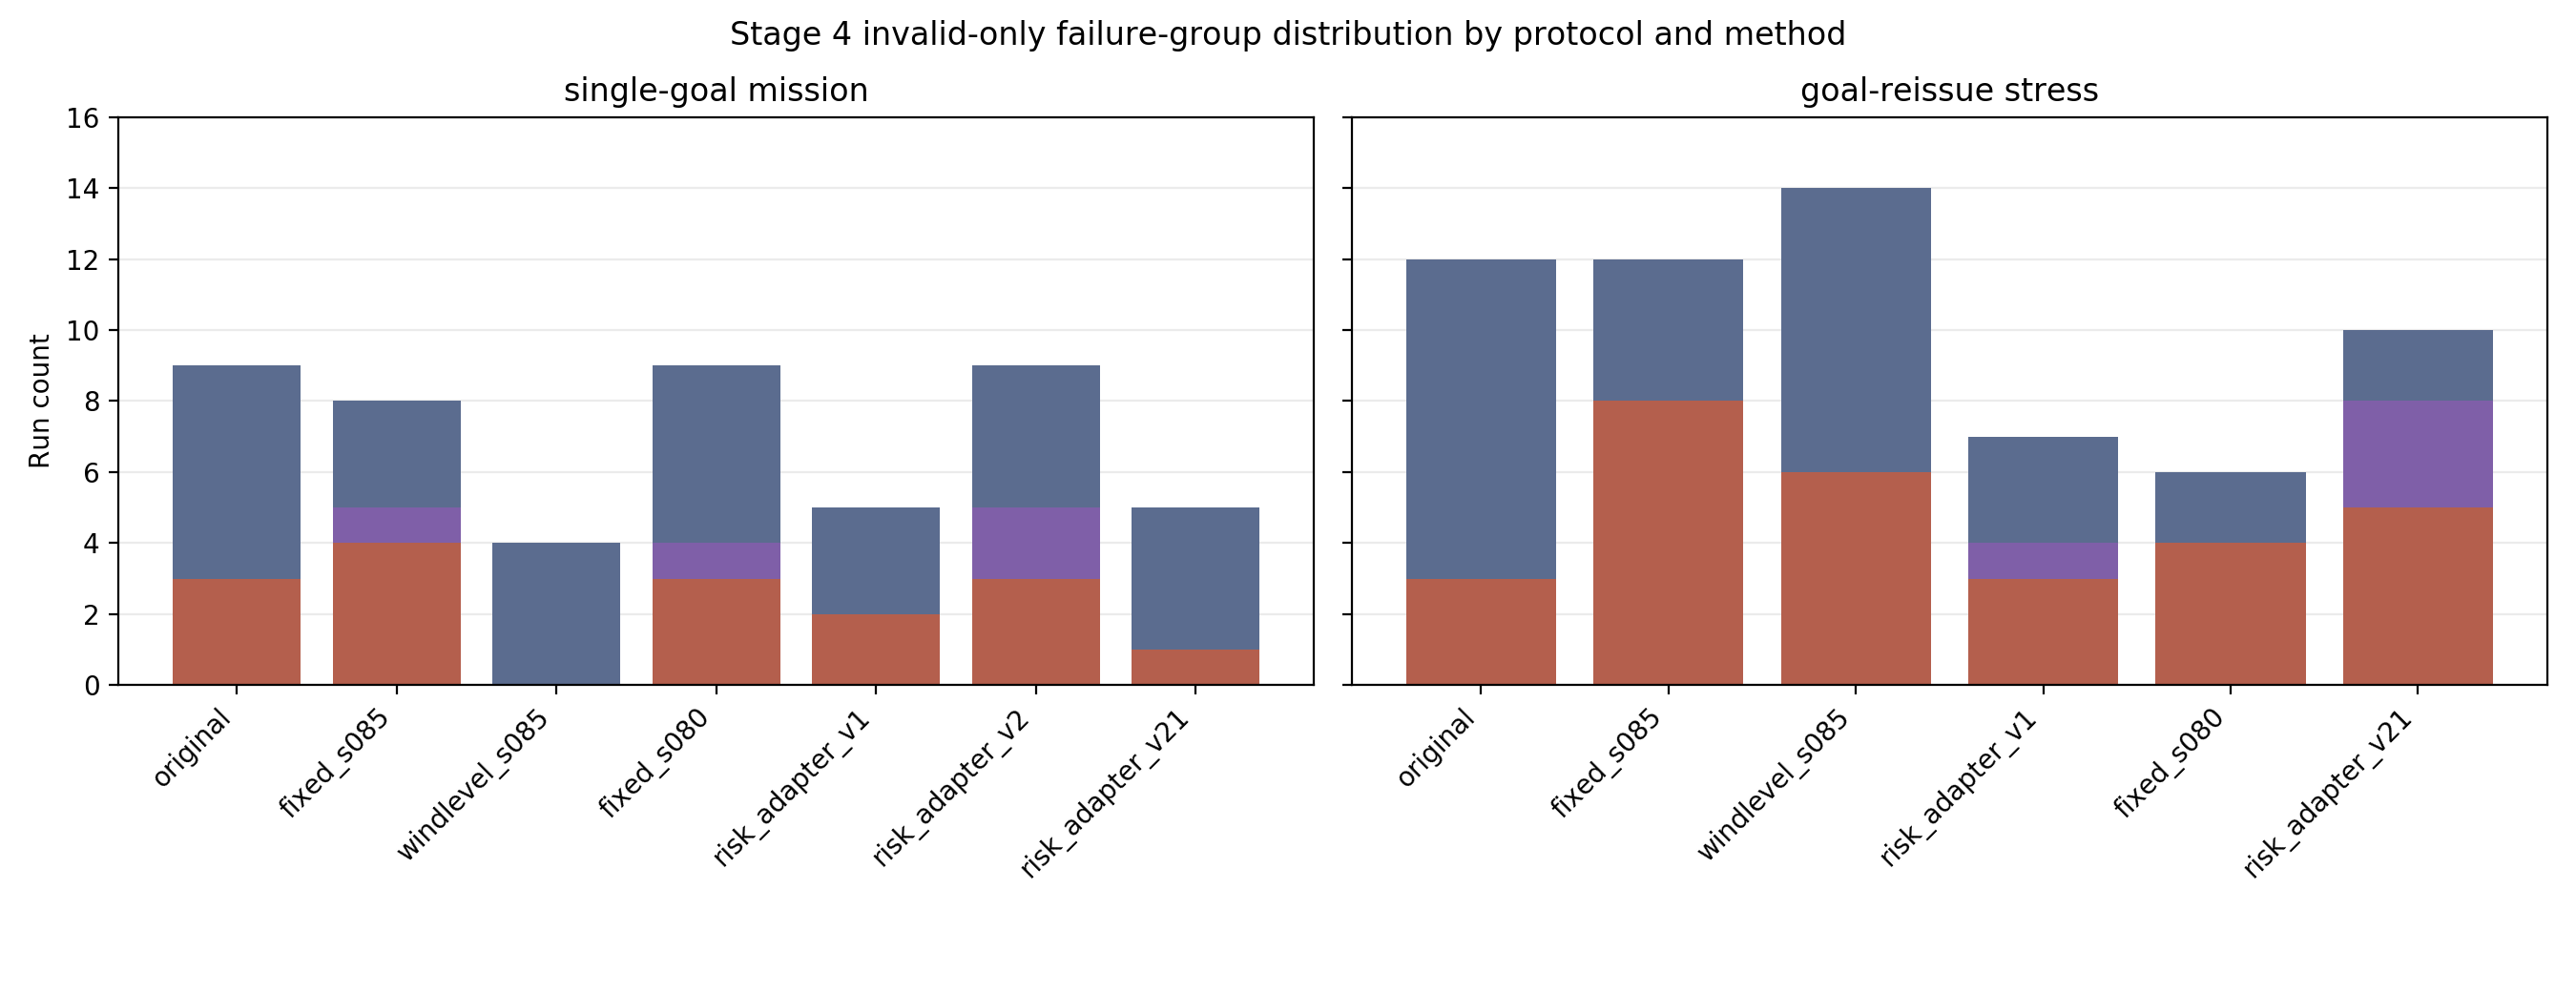
\includegraphics[width=\linewidth]{figures/fig5_invalid_failure_groups.png}
  \caption{Invalid-only failure groups. The categories expose heterogeneous
  failure patterns across protocols and methods, but they are diagnostic labels
  rather than definitive root-cause attribution.}
  \label{fig:failure_groups}
\end{figure}

In the goal-reissue stress protocol, Risk Adapter v2.1 shows larger
planner-reference and command/control components than Risk Adapter v1,
consistent with its weaker stress-protocol result. This diagnostic view
supports the reframed paper claim: aggregate strict-valid counts alone are
insufficient for interpreting robustness.

\subsection{Representative Trace Analysis}

Representative traces add a case-study view of the same trade-offs. In Trial 4
under goal-reissue stress, several Risk Adapter v2.1 failures occur
before arrival rather than only after post-arrival goal republishes. These
traces point to early pre-arrival vulnerability and risk availability or timing
issues, not merely a goal-reissue artifact. Trial 6 under the single-goal
protocol shows a different pattern: lower command scale is not automatically
safer, and delayed post-arrival divergence can still occur under
goal repeat = 1.

\begin{figure*}[t]
  \centering
  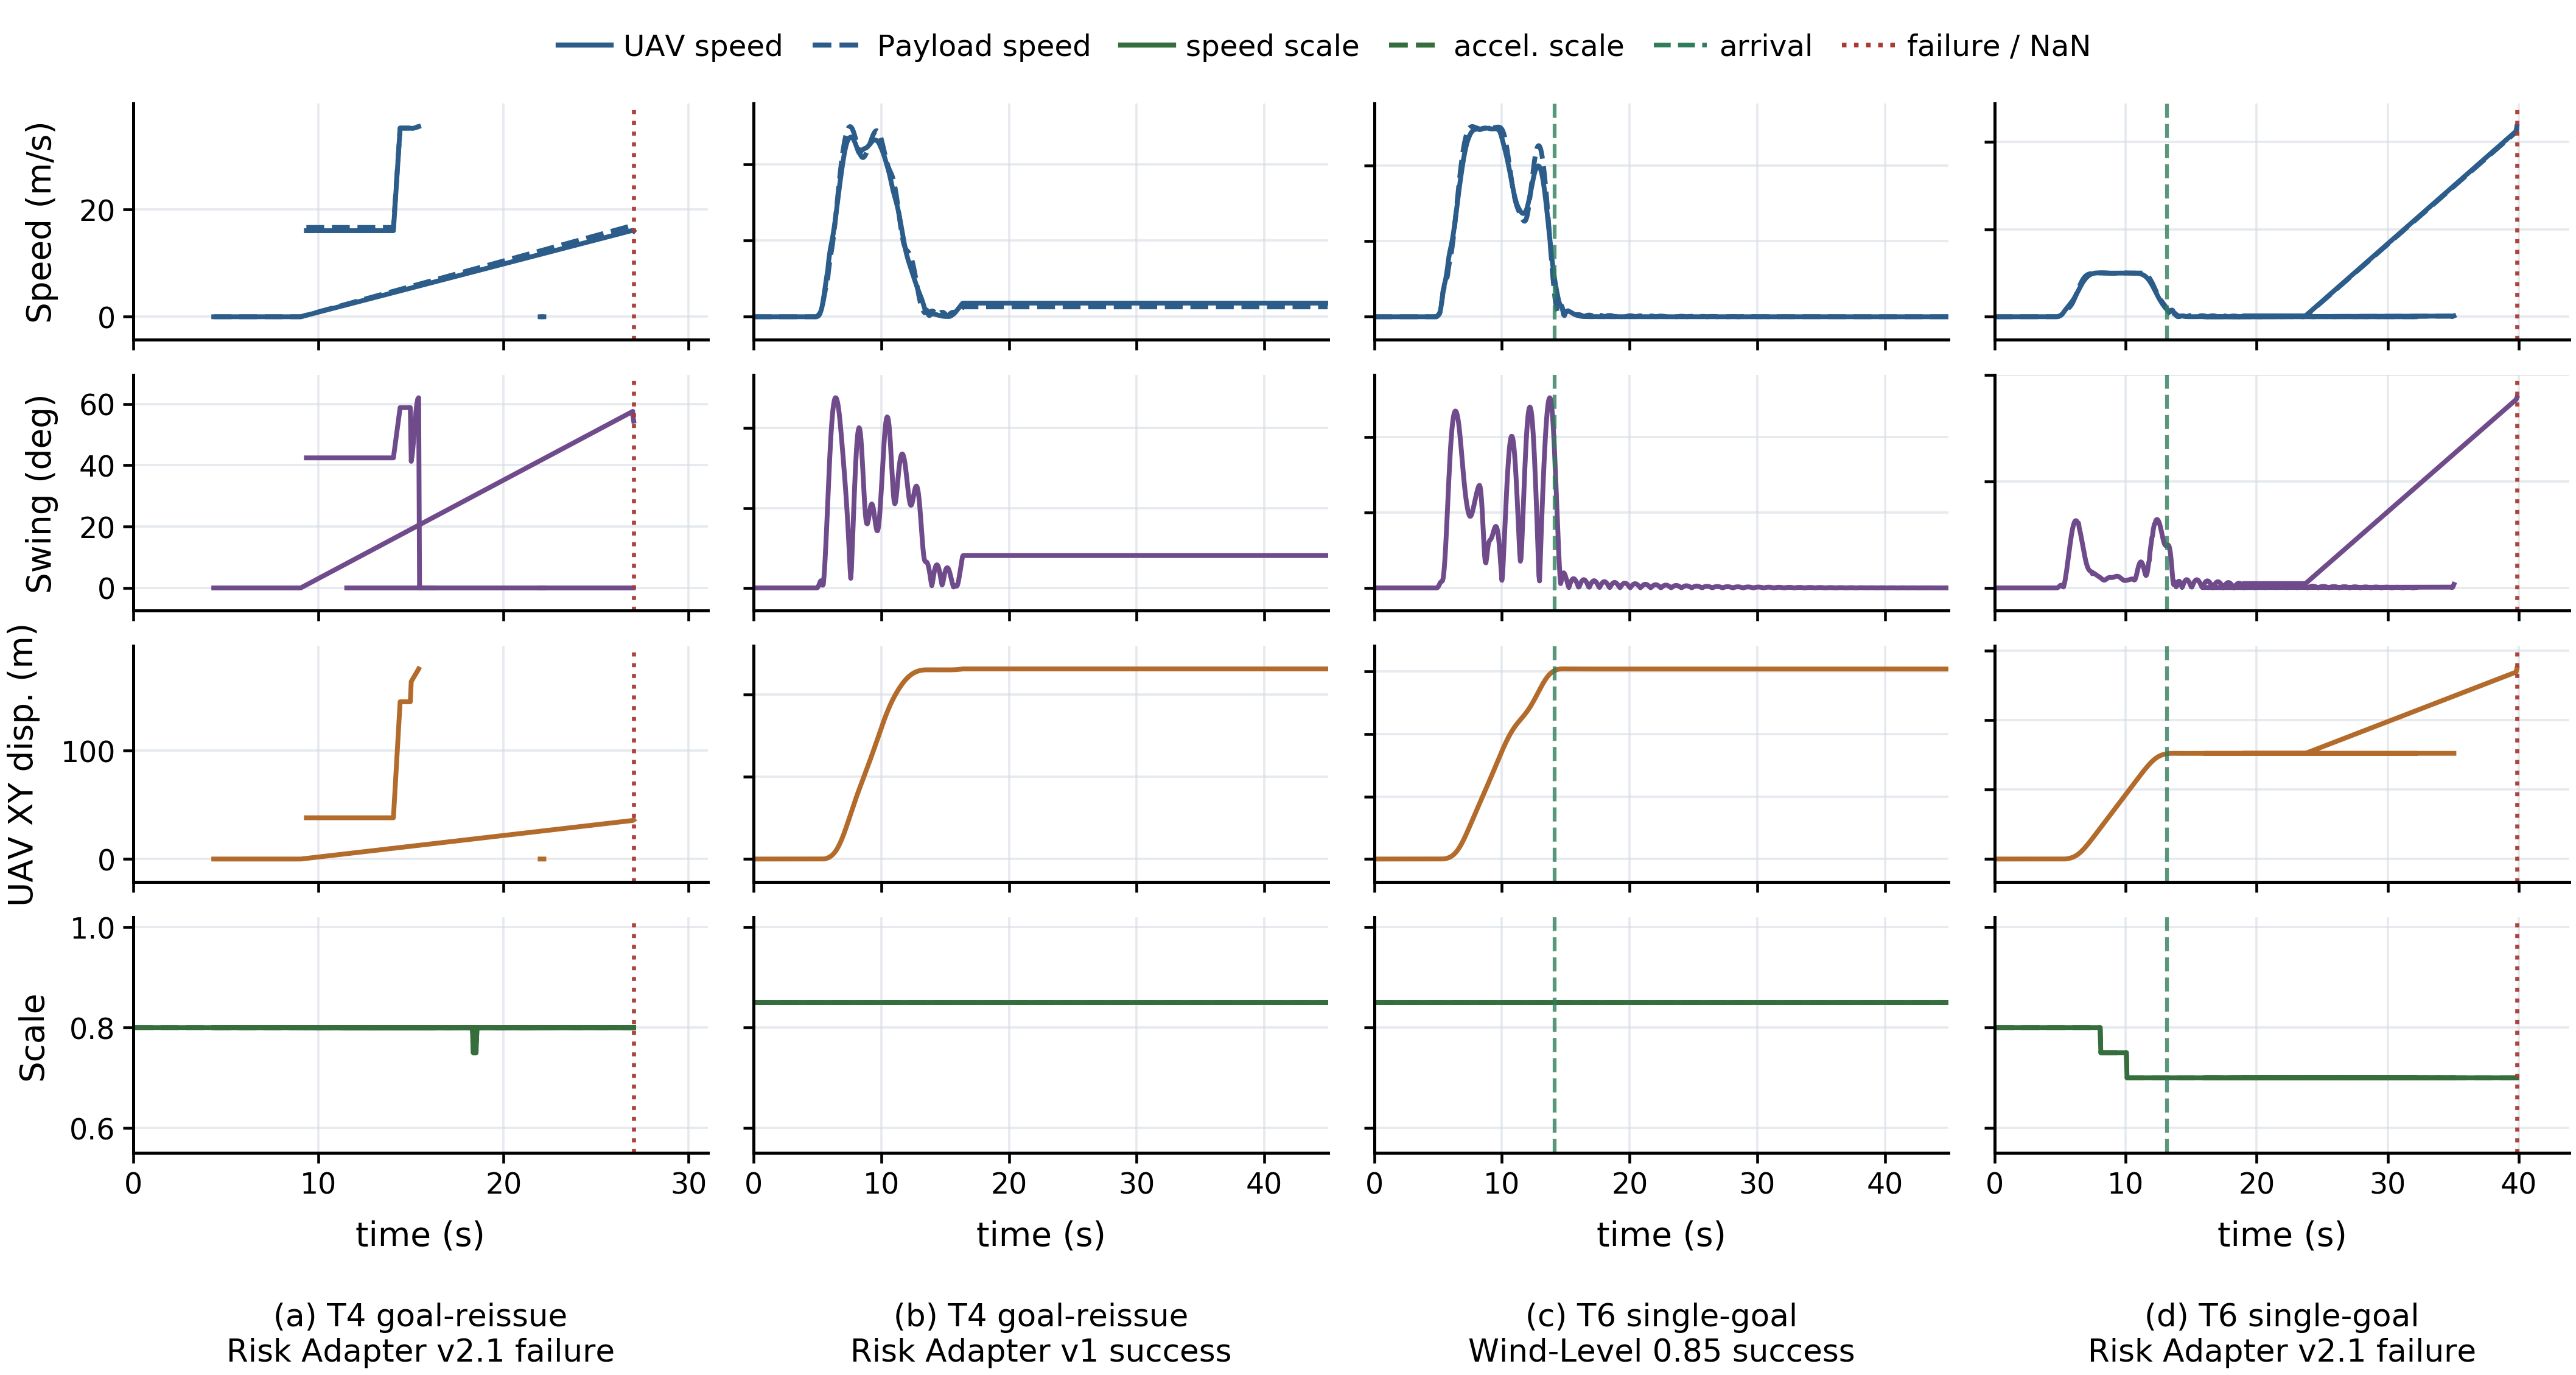
\includegraphics[width=\textwidth]{figures/fig6_trace_summary.png}
  \caption{Representative trace summary for selected failure and success
  cases. Columns compare Trial 4 goal-reissue stress and Trial 6 single-goal
  bottleneck behavior. The figure keeps only key speed, swing, UAV XY displacement, and
  governor-scale signals for readability. Full trace details are available in
  supplementary / archived trace assets. The traces are qualitative mechanism
  evidence, not proof of general causality.}
  \label{fig:representative_traces}
\end{figure*}

\subsection{Summary of Findings}

\begin{itemize}
  \item Simple baselines are strong protocol specialists:
  Wind-Level 0.85 leads the single-goal protocol and Fixed Scale 0.80 leads the
  goal-reissue stress protocol.
  \item Risk Adapter v1 is the most balanced current learned /
  risk-conditioned method by mean valid count, worst-protocol valid count, and
  total regret.
  \item Risk Adapter v2.1 improves nominal / single-goal behavior but is weaker
  under goal-reissue stress; Risk Adapter v1 matches its single-goal count and
  improves its stress count in the two-protocol plane.
  \item Protocol split and invalid-only failure groups are necessary to
  interpret robustness; a single combined aggregate would hide specialist
  trade-offs.
\end{itemize}
